\chapter{The VILLA Project: Methodology}\label{sec:2}

The present chapter presents an introduction to the VILLA project, with a specific focus on those aspects which are directly relevant for the object of the volume. A more detailed description of all other aspects may be found in \citet{DimrothEtAl2013} and the forthcoming VILLA manual (\citeauthor{WatorekEtAlND} in prep).

\section{The course}\label{sec:02:1}

The objective of the VILLA project was to observe the very earliest stages of the acquisition of a morphologically complex language in light of the input received. It follows that the input is a particularly crucial component of the project, as not only did it contain the raw material for language acquisition, but was also a carefully controlled independent variable in the experiment design. 

In order to maximise learner engagement and provide a realistic environment, the VILLA input was provided in the shape of a 14-hour interactive Polish course, taught by a native speaker specifically trained for that purpose. The same teacher worked in all editions of the VILLA project, moving across Europe to teach in the universities which took part in the initiative: Nijmegen (the Netherlands), Osnabrück (Germany), Paris VIII (France), York (UK), Pavia, Bergamo (Italy).

The research question of the VILLA project required that input should be thoroughly controlled for. Moreover, for the purposes of cross-linguistic comparison, it had to be kept as constant as possible across the various editions. To this end, input was planned in advance, and a course schedule was prepared for the teacher to follow in all editions. The course thus had a very precise structure, detailing the topics to cover, the vocabulary to introduce, the activities to perform, and, crucially, the frequency with which lexical items had to occur during classes. 

Although some slides included a few written words in Polish orthography, Polish orthographic conventions were never introduced, so that learners would have been hardly able to autonomously read them in a target-like manner. Nevertheless, it is quite possible that they tried to pair the words they heard in the input to their written representation in some of the slides used in the course (the only available source of written input).

As far as contents are concerned, the VILLA course describes a handful of characters (the members of the Kowalski family) in terms of nationality, address, family links, profession, likes and dislikes, home furniture etc. A specific section is devoted to the description of a map and to giving route directions. An unexhaustive list of the grammatical structures practices throughout the course includes copular structures, transitive constructions, prepositional phrases, nominal paradigms, various verb endings (infinitive, 3sg) etc.

It is important to point out that the VILLA input is much more varied than the target structure examined in this work, which is but one of the many grammatical constructions included in the course. Said otherwise, VILLA is not a psycho-linguistic experiment devoted exclusively to transitive structures, in which the input was only meant to provide the learners with the necessary examples. On the contrary, from the learner perspective the VILLA course was primarily a language course (albeit with a few peculiarities, such as the prohibition to take notes: see below) containing a wide variety of lexical items and grammatical structures, some of which were later tested in some of the project tasks.

In each country except Germany (where child and adult acquisition were compared), the same contents were organised into two versions of the input, namely meaning-based (MB) and form-based (FB). Although only the results relative to the former (including the German adult group) are discussed in this work, it is worthwhile to briefly describe both types of input so as to highlight the main differences, designed in order to pursue research questions concerning the factors influencing input saliency. 

The purpose of the MB input is to avoid drawing the learner’s attention on any particular feature of Polish. \figref{fig:02:1} shows a typical slide from the MB input course focussing on transitive structures such as \textit{Eryk lubi kawę} ‘Eryk.\textsc{nom} likes coffee.\textsc{acc}’. As can be seen, no written word-forms or hints of any kind as to the target structure (the accusative case) are presented. Learners of the MB editions could only rely on their own processing skills in order to identify and organise any formal regularities of the aural and written input.

\begin{figure}
    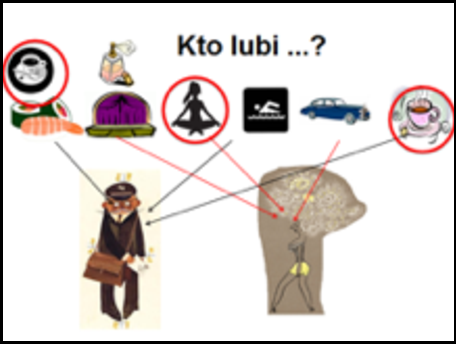
\includegraphics[width=\textwidth]{figures/02-1.pdf}
    \caption{MB input example slide}
    \label{fig:02:1}
\end{figure}

In contrast, the FB groups were exposed to enhanced input (\citealt{Sharwood-Smith1993}), designed to highlight specific formal features of the input. This was mainly achieved through focus-on-form activities (\citealt{DoughtyWilliams1998}) and corrective feedback. Linguistic information was visually presented in a more explicit fashion, as exemplified in \figref{fig:02:2}.

\begin{figure}
    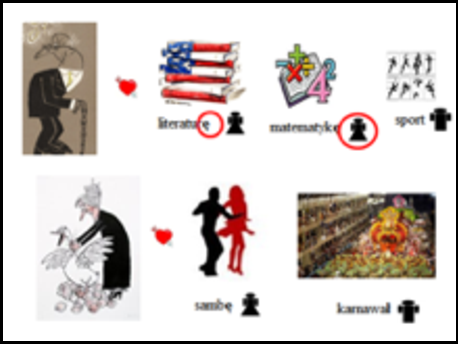
\includegraphics[width=\textwidth]{figures/02-2.pdf}
    \caption{MB input example slide}
    \label{fig:02:2}
\end{figure}

The slide focuses on transitive constructions, but the written word-forms of target items are presented on screen and graphically highlighted (the \textit{–ę} ending, here circled in red) together with other relevant information, such as the grammatical gender of the referent (the “feminine” icon, also  circled in red). Thus, learners are provided with a complete set of meta-linguistic information. Nevertheless, even the FB input includes no metalanguage and students were never provided with explicit \textit{explanations} as to the target grammar. 

Beside these differences, the input contents were the same for both groups. In addition ot the range of lexical items and grammatical structures, their frequency and order of appearance in particular were kept as uniform as possible. 

\subsection{Input control}\label{sec:02:1.1}

As stated in the introduction, one of the major objectives of the VILLA project was a detailed, fine-grained analysis of the relation between input and intake. It is clear that thorough input control is an essential prerequisite in order to pursue this research question. In the VILLA project this ambitious objective required several steps.

First, one had to control for the participants’ existing experience of the target language. This was  only possible through the exclusion of participants who declared any previous contacts with Polish or other Slavic languages. Second, it was necessary to make sure that exposure to Polish throughout the course would be limited to the experimental input, including teacher speech and a set of PowerPoint slides. The choice of Polish as a target language made it rather unlikely that participants could accidentally be exposed to it outside classes. In any case, all participants signed a contract to the effect that they would not intentionally look for additional information on Polish. Clearly it is impossible to verify whether or not this requirement was respected.

In order to make the experimental input as uniform as possible in terms of both quantity and quality, learners were asked not to take notes during classes. The rationale behind this decision is that the quality of learners’ notes as well as their effort would very likely differ from person to person, thus introducing an undesirable variable beyond methodological control. For the same reason, no homework was assigned and individual practice outside classes was discouraged.

Finally, input was carefully planned in terms of topics, vocabulary and frequency of both lexical items and syntactic structures. This resulted in a general scheme which the teacher replicated with remarkable accuracy throughout the various editions of the course. Classes would never be identical to each other, as they were not recorded but performed live. Nevertheless, since frequency was one of the variables controlled for in the tests, it was vital that the target linguistic items should occur an equal number of times in each edition. To this aim, classes were monitored in real time by a team member, who signalled to the teacher whether a given word had appeared too rarely or too often in relation to its planned frequency. An \textit{a posteriori} analysis on the input corpus showed that lexical frequencies were indeed comparable across the editions of the VILLA project, which is a real credit to the teacher for managing to maintain consistency over ten different courses and a time span of almost a year.

\subsection{Input transcription}\label{sec:02:1.2}

By far the most thorough tool of input control was input recording and transcription, so that it can now be accessed and studied in a written format. The teacher wore a portable wireless microphone which recorded her speech. The resulting tracks were subsequently transcribed\footnote{The input for Italian and English editions was transcribed by Jacopo Saturno; the French, German and Dutch editions were  transcribed by members of the corresponding research teams.} in standard orthography using ELAN (\citealt{BrugmanRussell2004}). This software makes it possible to time-align transcriptions, i.e. to automatically associate each annotation with the corresponding audio segment (\figref{fig:02:2}). Transcription is produced from left to right along the horizontal axis; participants are assigned different tiers which are listed from top to bottom.

\begin{figure}
    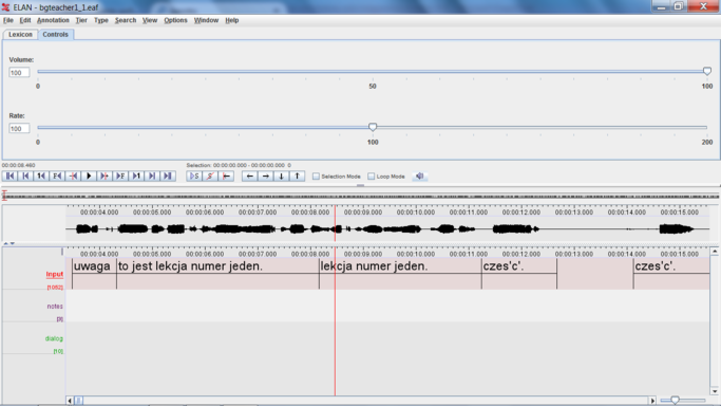
\includegraphics[width=\textwidth]{figures/02-3.pdf}
    \caption{transcription of the VILLA input with ELAN}
    \label{fig:02:3}
\end{figure}

To separate input addressed to all learners from comments aimed at individual learners or groups during interactional games, teacher speech was transcribed on two different tiers, labelled *TEA and *TEB respectively. Since it represents the vast majority of utterances, only the former is considered in this work. The ELAN files were converted into a text-like top-bottom format using the CHAT/CLAN \citep{MacWhinney2000} suite of software (\figref{fig:02:4}).
% \begin{figure}
%     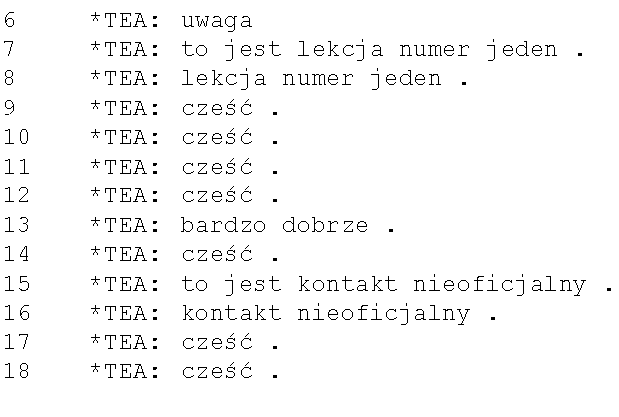
\includegraphics[width=\textwidth]{figures/02-4.pdf}
%     \caption{transcription of the VILLA input in CHAT}
%     \label{fig:02:4}
% \end{figure}

\begin{table}
\ttfamily
    \begin{tabular}{lrl}
        6    &   *TEA: & uwaga\\
        7    &   *TEA: & to jestlekcjanumerjeden . \\
        8    &   *TEA: & lekcjanumerjeden .  \\
        9    &   *TEA: & cześć .  \\
        10   &   *TEA: & cześć .  \\
        11   &   *TEA: & cześć .  \\
        12   &   *TEA: & cześć .  \\
        13   &   *TEA: & bardzodobrze .  \\
        14   &   *TEA: & cześć .  \\
        15   &   *TEA: & to jestkontaktnieoficjalny .  \\
        16   &   *TEA: & kontaktnieoficjalny .  \\
        17   &   *TEA: & cześć .  \\
        18   &   *TEA: & cześć . \\
    \end{tabular}
    \caption{transcription of the VILLA input in CHAT}
    \label{fig:02:4}
\end{table}

A CHAT-CLAN automatic morphological tagging system was developed by Christine Dimroth and Roman Skiba, with a small contribution by the present author (\figref{fig:02:5}). 

% \begin{figure}
%     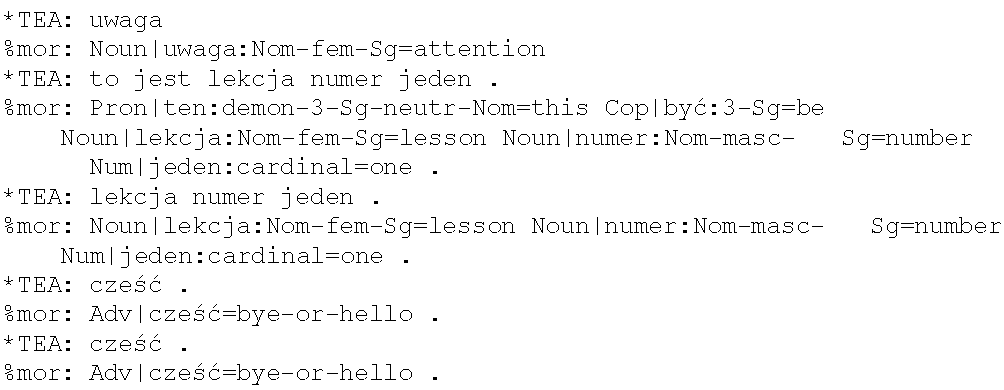
\includegraphics[width=\textwidth]{figures/02-5.pdf}
%     \caption{automatic morphological tagging of the VILLA input in CHAT}
%     \label{fig:02:5}
% \end{figure}

\begin{table}
\ttfamily
    \begin{tabular}{ll}
        *TEA:   & uwaga\\
        \%mor:  & Noun|uwaga:Nom-fem-Sg=attention\\
        *TEA:   & to jestlekcjanumerjeden . \\
        \%mor:  & Pron|ten:demon-3-Sg-neutr-Nom=this Cop|być:3-Sg=be \\
        ~       & Noun|lekcja:Nom-fem-Sg=lessonNoun|numer:Nom-masc-Sg=number\\
        ~       & Num|jeden:cardinal=one . \\
        *TEA:   & lekcjanumerjeden .  \\
        \%mor:  & Noun|lekcja:Nom-fem-Sg=lessonNoun|numer:Nom-masc-Sg=number\\
        ~       & Num|jeden:cardinal=one . \\
        *TEA:   & cześć .  \\
        \%mor:  & Adv|cześć=bye-or-hello . \\
        *TEA:   & cześć .  \\
        \%mor:  & Adv|cześć=bye-or-hello . \\
    \end{tabular}
    \caption{automatic morphological tagging of the VILLA input in CHAT}
    \label{fig:02:5}
\end{table}

On the dependent tier \%mor, each word is morphologically tagged with the appropriate values of the relevant grammatical categories, depending on the word class considered (e.g. case, gender, number and lexeme for nouns; person, number and lexeme for verbs, and so on). To each item in the original transcript, the CLAN Mor programme associates the appropriate gloss, retrieving it from a specially designed lexicon. In case a given form corresponds to more than one tag, which because of widespread morphological syncretism is a fairly common case in Polish, all tags are presented subsequently. Glosses were not disambiguated in any way.

Building on that basis  a similar yet separate system was developed for the purposes of the present work by adapting the same principle to a different tool, namely the software R (\citealt{RCoreTeam2017}) and its package \textit{stringr} \citep{Wickham2017}. New labels (in Italian) were also devised for all grammatical categories, such as verbs, pronouns and adjectives. Compared to the system presented above, this new version facilitates frequency searches for morphosyntactic patterns in several technical respects.

Again, tags may include more than one possible grammatical meaning, as exemplified in \REF{ex:02:1}.

\ea%1
    \label{ex:02:1}
    \textit{balonik}:sostantivoIN\_Acc\_Mas\_Sg//sostantivoIN\_Nom\_Mas\_Sg:balonik
    \z

The input transcript, once glossed, can be searched for appropriate patterns through regular expressions. A search for SVO sentences with animate masculine nouns as subject and inanimate feminine nouns as object, for example, should retrieve hits like \textit{Leon} \textit{lubi} \textit{herbatę}, ‘Leon likes tea’. In addition, it is possible to identify all the instances of a given lexeme or grammatical value such as, for example, ‘nominative masculine singular’. This possibility will be widely exploited in \chapref{sec:3}, in which searches were performed using R (\citealt{RCoreTeam2017}) and its package \textit{stringr} \citep{Wickham2017}.

\subsection{The VILLA input as a variety of Polish}\label{sec:02:1.3}

While the VILLA project uses a natural language as input, it would be imprecise to claim that the input provided by the teacher could be a representative example of native varieties. This is quite natural if one takes into account the peculiar context in which the experiment took place, including its time span, which was limited to 14 hours, and the research questions regarding the role of input, which could only be answered by manipulating it. These constraints result in a language variety which at times may sound a little odd to a native speaker of Polish. 

First, the dramatic competence gap between the teacher and the total beginner learners often results in a register definable as Teacher talk (\citealt[134–144]{Larsen-FreemanLong1991}) whose purpose is to simplify the input as much as possible while maintaining grammatical correctness. In fact, teacher speech within the VILLA project was extremely slow and hyperarticulated in an effort to make input more salient, i.e. more easily perceivable and segmentable. 

Second, the choice was made to focus on a limited number of target structures, whose acquisition was later probed through the linguistic tasks. This caused them to be often produced with unnatural frequency, as is the case for the copula verb \textit{jest} ‘is’. Further, the frequency of syntactic structures directly conditions the frequency of the inflected word-forms belonging to the paradigm of a word. Compared to native varieties, input manipulation results in only a limited number of word-forms being represented in the VILLA input: plural forms for instance are completely absent for most nouns. Even within the singular number, the VILLA input is much more restricted than any L1 variety, being limited to only a couple of forms. Depending on the type of noun, the input might focus on the opposition between NOM and INS, for animate nouns, or between NOM and ACC, for inanimate ones. While most nouns only occurred in one or two forms, some did show a greater range of morphological endings. 

Copular structures usefully illustrate another source of deviations from native varieties, namely pragmatics. Two main types of predicational copular clauses may be distinguished in Polish \citep{Bondaruk2013}: In NOM-type structures (following the labels introduced in \citealt{Saturno2015}), the invariable pronoun \textit{to} ‘this’ is supplied independently of referent gender and number, while the complement appears in the nominative form, e.g. \textit{to} \textit{jest} \textit{Filip} ‘this is Filip’. INS-type structures, in contrast, require the personal pronoun \textit{on} ‘he’ or \textit{ona} ‘she’, which specify the gender of the corresponding referent, while the noun is provided in the instrumental case, e.g. \textit{on jest studentem} ‘he is a student’.

In native varieties of Polish, the two structures are pragmatically differentiated. NOM-type structures are mainly used deictically in order to introduce new referents in the discourse, e.g. \textit{a to, kto to jest?} ‘and this [person], who is this [person]?’. In contrast, the personal pronouns of INS-type structures typically refer to entities in an anaphoric manner, which means that the referent is already part of the discourse: the copular structure is used to provide additional details, e.g. \textit{kim on jest?} ‘who is he? [what's his job/nationality etc]?’. In contrast, in the VILLA input the two structures are used quite interchangeably in all contexts, so that no functional differentiation applies. Example \REF{ex:02:2}, extracted from the teacher's speech, shows that the two structures may be used to refer to the same entity in the same context. The teacher first asks (rhetorically) who Karol is using a an INS-type copular structure \REF{ex:02:2a}, which calls for the same structure in the responses in \REF{ex:02:2b} and \REF{ex:02:2c}. However, in \REF{ex:02:2d} the teacher switches to a NOM-type copular structure, in which the noun appears in the nominative case and the referent is deictically instantiated by the invariable pronoun \textit{to}, ‘this’. While this structure is grammatically correct, it would sound pragmatically inappropriate to a native speaker of Polish.

\ea%2
    \label{ex:02:2}
    \ea\label{ex:02:2a}
    \gll    A Karol, kim jest Karol?\\
            and Karol.\textsc{nom} who.\textsc{ins} is Karol.\textsc{nom}?\\
    \glt    ‘And Karol, who is Karol?’
    \ex\label{ex:02:2b}
    \gll    Karol jest stra\.{z}akiem.\\
            Karol.\textsc{nom} is fireman.\textsc{ins}\\
    \glt    ‘Karol is a fireman.’
    \ex\label{ex:02:2c}
    \gll    On jest stra\.{z}akiem.\\
            he is fireman.\textsc{ins}\\
    \glt    ‘He is a fireman.’
    \ex\label{ex:02:2d}
    \gll    To jest stra\.{z}ak.\\
            this is fireman.\textsc{nom}\\
    \glt    ‘This is a fireman.’
    \z
\z

Similar structures were produced intentionally for didactic purposes, i.e. in order to show learners that predications about referents may be expressed through different syntactic constructions. This contrast was also the target structure of several tasks. Most VILLA research questions are concerned with morphosyntax, which in light of the constraints imposed by a first exposure study necessarily led to a partial neglect of pragmatics and information structure. While this state of things seemed inevitable for methodological reasons, it has two negative consequences: first, as mentioned, the input at times might seem unnatural to a native speaker of Polish; second, the two contrasting structures end up to express exactly the same meaning, so that the contrast loses any functional motivation.

Similar arguments may be made concerning a crucial point of the present work, namely the order of subject and object in transitive sentences. Although both SO and OS orders are possible in Polish, this does not mean that different versions carry an identical meaning, at least from a pragmatic point of view \citep{Siewierska1993}. In general terms, the first position in the utterance is associated with the topic function, so that moving the object to that position from its canonical post-verbal position equals to treating the subject as the focus and the object as the topic. This is not necessarily the case in the VILLA input, as example \REF{ex:02:3} makes clear.

\ea%3
    \label{ex:02:3}
    \ea\label{ex:02:3a}
    \gll    Filip wózek ciągnie.\\
            Filip.\textsc{nom} cart.\textsc{acc} pulls\\
    \glt    ‘Filip pulls the cart.’
    \ex\label{ex:02:3b}
    \gll    Filip ciągnie wózek tak.\\
            Filip.\textsc{nom} pulls cart.\textsc{acc} yes.\\
    \glt    ‘Filip pulls the cart.’
    \ex\label{ex:02:3c}
    \gll    Wózek ciągnie Filip.\\
            cart.\textsc{acc} pulls Filip.\textsc{nom}\\
    \glt    ‘Filip pulls the cart.’
    \z
\z

Compared to L1 practice, several facts are a little odd. First, the same referent is verbalised three times using maximally explicit means such as a person name. Second, based on the pragmatics of native Polish, one should conclude that \REF{ex:02:3a} focuses the verb, as in ‘Filip doesn't push the cart, he pulls it’; \REF{ex:02:3b}, at least in the absence of specific intonational patterns, should be interpreted as unmarked; in \REF{ex:02:3c}, finally, the focus would be on the subject, as in ‘it's not Julia who pulls the cart: it is Filip’. However, none of these interpretations is warranted in the example in question.

In fact, this obvious manipulation of syntax served the sole purpose of showing the learners that Polish word order is free. Unfortunately, given the very limited scope and vocabulary range of the VILLA project, at times it was impossible to do so in a pragmatically meaningful way, and the important link between information structure and syntax had to be sacrificed. On the one hand, word order manipulation was functional to research questions concerning cross-linguistic interference, such as “will speakers of rigidly SO languages be able to recognise and, perhaps, exploit Polish free word order?”. On the other hand, it could be argued that the purpose of word order manipulation, i.e. the expression of pragmatically marked meaning, could not be adequately inferred from the examples provided. 

In spite of these small differences with native varieties, it would be inappropriate to state that the VILLA Polish differs significantly from native varieties, or that it is not a natural language. The VILLA input retains numerous idiosyncrasies which are likely to create difficulties to the learners, and at the same time resemble the difficulties often encountered in SLA. Alongside a few instances of \textit{pluralia tantum}, several nominal paradigms present a range of idiosyncrasies and specificities which may not be immediately easy for the learner to grasp, such as the animacy-based differential object marking found in the paradigm of masculine nouns (see next section). To summarise, the VILLA input represents a specific variety of Polish, which retains the complexities and idiosyncrasies of a natural language, although it does present a limited range of lexical and grammatical items as well as a few instances in which syntax and pragmatics were somewhat bent to the need of didactics.

\section{The target language and the VILLA L1S}\label{sec:02:2}
\subsection{Inflectional morphology}\label{sec:02:2.1}

In addition to its low availability outside the language classroom in the countries where the VILLA courses were held, Polish was chosen as the target language of the experiment because it typologically differs from the VILLA L1s in various respects. One key feature is its rich and complex system of nominal morphology, contrasting two numbers, three genders in the singular and two in the plural, and crucially, as many as seven cases. \tabref{tab:02:1} shows the paradigms which appear in the VILLA input. Virtually all nouns appeared in the singular number only, so much so that plural forms may be considered exceptional (they are mainly limited to a few \textit{pluralia tantum}) and will not be considered in this volume.

\begin{table}
    \begin{tabular}{llllll}
\lsptoprule
         & M ANIM & F ANIM & M INANIM & F INANIM & NEU\\
\midrule
        NOM & strażak & mam-a & balonik & kaw-a & biurk-o\\
        GEN & strażak-a & mam-y & balonik-u & kaw-y & biurk-a\\
        DAT & strażak-owi & mam-ie & balonik-owi & kaw-e & biurk-owi\\
        ACC & strażak-a & mam-ę & balonik & kaw-ę & biurk-o\\
        INS & strażak-iem & mam-ą & balonik-iem & kaw-ą & biurk-iem\\
        LOC & strażak-u & mam-ie & balonik-u & kaw-ie & biurk-u\\
        VOC & strażak-u & mam-o & balonik-u & kaw-o & biurk-o\\
        & ‘fireman’ & ‘grandmother’ & ‘balloon’ & ‘coffee’ & ‘desk’\\
\lspbottomrule
    \end{tabular}
    \caption{Polish nominal paradigm, singular}
    \label{tab:02:1}
\end{table}

The selection of the ACC ending depends on the interaction of animacy and grammatical gender, defined by noun-adjective agreement and NOM ending. Animacy is not relevant in the case of neuter and feminine nouns (\ref{ex:02:4a} and \ref{ex:02:4b}), but it determines whether the ACC of masculine nouns is identical to the NOM in non-palatalized consonant, as for inanimate nouns \REF{ex:02:4c}, or, in the case of animate nouns \REF{ex:02:4d}, to the genitive in \textit{-a} \REF{ex:02:4e}.

\ea%4
    \label{ex:02:4}
    \ea\label{ex:02:4a}
    \gll    Jan-${\emptyset}$ lubi kaw-ę\\
            Jan-\textsc{nom}  likes    coffee.\textsc{f}-\textsc{acc}\\
    \ex\label{ex:02:4b}
    \gll    Jan-${\emptyset}$ kocha mam-ę\\
            Jan-\textsc{nom} loves sister.\textsc{f-acc}\\
    \ex\label{ex:02:4c}
    \gll    Jan-${\emptyset}$ ma balonik-${\emptyset}$\\
            Jan-\textsc{nom} has balloon.\textsc{m-acc}\\
    \ex\label{ex:02:4d}
    \gll    Jan-${\emptyset}$ zna strażak-a\\
            Jan-\textsc{nom} knows fireman.\textsc{m-acc}\\
    \ex\label{ex:02:4e}
    \gll    to jest samochód-${\emptyset}$ strażaka\\
            this.\textsc{nom}  is  car-\textsc{nom}  fireman.\textsc{gen}\\
    \z
\z

Syncretism may obscure the one-to-one pairing of form and function. Even in a subset of Polish as is represented in the VILLA input, the inflectional ending -a expresses at least two types of grammatical meaning in the nominal domain, i.e. NOM.F and GEN/ACC.M (the latter for animate nouns only), in addition to the 3sg of some verbs (e.g. \textit{on zna} ‘he knows’). Whenever instances of such categories co-occur, they present the same ending \REF{ex:02:5}. It follows that in order to apply the morphosyntactic principle of utterance decoding, the listener needs to be aware of the grammatical gender of the nouns involved as well as their inflectional paradigm.

\ea%5
    \label{ex:02:5}
    \gll    siostr-a lubi brat-a\\
            sister-\textsc{nom}  likes  brother-\textsc{acc}\\
    \z

In terms of inflectional morphology, the VILLA L1 closest to Polish is certainly German. This is the only L1 to express case on nouns, while all others only distinguish case on some personal pronouns. However, case in German is mainly signalled on the determiner (completely absent in Polish), while the inflectional paradigm is characterised by diffused syncretism, whereby several functionally differentiated word-forms are formally identical (\tabref{tab:02:2}). Indeed, it has been shown (\citealt{KempeMacWhinney1998, KempeMacWhinney1999} for Russian) that the Slavic case is a much better cue to the identification of the sentence agent than it is in German, for both native speakers and learners.

\begin{table}
    \begin{tabularx}{\textwidth}{lXll}
    \lsptoprule
        \multicolumn{1}{c}{} &  & M & F\\
    \midrule
        \multicolumn{1}{c}{SING} & NOM & der Feuerwehrmann & die Köch-e\\
        & GEN & des Feuerwehrmann-s & der Köch-e\\
         & DAT & dem Feuerwehrmann & den Köch-en\\
         & ACC & den Feuerwehrmann & die Köch-e\\
        \multicolumn{1}{c}{PLUR} & NOM & die Feuerwehrmänn-er & die Köchinn-en\\
        & GEN & der Feuerwehrmänn-er & der Köchinn-en\\
         & DAT & der Feuerwehrmänn-ern & den Köchinn-en\\
         & ACC & die Feuerwehrmänn-er & die Köchinn-en\\
        \multicolumn{1}{c}{} &  & ‘fireman’ & ‘cook(F) ‘\\
\lspbottomrule
    \end{tabularx}
    \caption{German nominal inflection}
    \label{tab:02:2}
\end{table}

The four remaining L1s, namely Dutch (\tabref{tab:02:3}), Italian (\tabref{tab:02:4}), French (\tabref{tab:02:5}) and English (\tabref{tab:02:6}) lack case altogether as far as nouns are concerned. These only present two forms, corresponding to singular and plural.

\begin{table}
    \begin{tabularx}{\textwidth}{XX@{\hspace{1cm}}Xl}
    \lsptoprule
        \multicolumn{2}{c}{Singular} & \multicolumn{2}{c}{Plural}\\
    \midrule
        M & F & M & F\\
        de kok & de kokkin & de kok-s & de kokkin-s, kokkinn-en\\
        ‘the fireman’ & ‘the cook.\textsc{f}’ & ‘the firemen’ & ‘the cooks.\textsc{f}’\\
\lspbottomrule
    \end{tabularx}
    \caption{Dutch nominal inflection}
    \label{tab:02:3}
\end{table}

\begin{table}
    \begin{tabularx}{\textwidth}{XX@{\hspace{1cm}}Xl}
    \lsptoprule
        \multicolumn{2}{c}{Singular} & \multicolumn{2}{c}{Plural}\\
    \midrule
        F & M & F & M\\
        il pompier-e & la cuoc-a & i pompier-i & le cuoch-e \\
        ‘the fireman’ & ‘the cook.\textsc{f}’ & ‘the firemen’ & ‘the cooks.\textsc{f}’\\
\lspbottomrule
    \end{tabularx}
    \caption{Italian nominal inflection}
    \label{tab:02:4}
\end{table}

The cases of French and English are particularly extreme. Regarding the former, even the singular and plural forms of nouns are only distinguishable in the written variety, as they are completely homophonous in speech: the only morphological cue to number is the determiner (\tabref{tab:02:5}).

\begin{table}
    \begin{tabularx}{\textwidth}{XX@{\hspace{1cm}}Xl}
    \lsptoprule
        \multicolumn{2}{c}{Singular} & \multicolumn{2}{c}{Plural}\\
    \midrule
        M & F & M & F\\
        \textit{le} \textit{pompier} & \textit{la} \textit{cuisinière} & \textit{les} \textit{pompiers} & \textit{les} \textit{cuisinières}\\
        {\textbackslash}lə p\~{ɔ}.pje{\textbackslash} & {\textbackslash}la kɥi.zi.njɛʁ{\textbackslash} & {\textbackslash}le p\~{ɔ}.pje{\textbackslash} & {\textbackslash}le kɥi.zi.njɛʁ{\textbackslash}\\
        ‘the fireman’ & ‘the cook.\textsc{f}’ & ‘the firemen’ & ‘the cooks.\textsc{f}’\\
\lspbottomrule
    \end{tabularx}
    \todo[inline]{// instead of {\textbackslash}{\textbackslash}?}
    \caption{French nominal inflection}
    \label{tab:02:5}
\end{table}

Gender is not morphologically encoded in English nouns, which only distinguish a singular and a plural form. Even when a noun is characterised in terms of intrinsic sex, this category is only visible through anaphoric reference.

\begin{table}
    \begin{tabularx}{\textwidth}{ll@{\hspace{1cm}}ll}
    \lsptoprule
        \multicolumn{2}{c}{Singular} & \multicolumn{2}{c}{Plural}\\
    \midrule
        \textit{the} \textit{fireman} & \textit{the} \textit{cook} & \textit{the} \textit{firemen} & \textit{the} \textit{cook-s}\\
\lspbottomrule
    \end{tabularx}
    \caption{English nominal inflection}
    \label{tab:02:6}
\end{table}


As far as word order is concerned, Polish is a predominantly SVO language \citep{Dryer2013a}, although the encoding of case makes it possible to freely manipulate it for pragmatic purposes. Word order in German may also be manipulated for pragmatic reasons without the need for specific syntactic devices (such as cleft sentences), because syntactic functions are made explicit by case marking. It is worth noting that, unlike Polish, German word order is constrained by the obligatoriness of the finite verb in second position.

In all VILLA L1s except German, the lack of explicit case marking results in syntactic functions being assigned based on the default SO word order. Departures from this pattern \REF{ex:02:6a} are possible, but require marked phonological or syntactic means, particular intonational contours, cleft sentences \REF{ex:02:6b} or dislocations \REF{ex:02:6c}. Of course, all these possibilities are also available in languages with more complex morphology, like Polish \REF{ex:02:6d}. Word order manipulation in these languages is simply an extra resource to explicitly mark information structure \REF{ex:02:6e}, but this does not immediately translate into their being more flexible, or favouring more variable word orders. 

\ea%6
    \label{ex:02:6}
    \ea\label{ex:02:6a}
    \gll    il gatto insegue il cane\\
            \textsc{art.m.sg}  cat  chases \textsc{art.m.sg} dog\\
    \ex\label{ex:02:6b}
    \gll    è il gatto che insegue il cane\\
            is  \textsc{det.m.sg}  cat  \textsc{rel}  chases    \textsc{art.m.sg}  dog\\
    \ex\label{ex:02:6c}
    \gll    il cane lo insegue il gatto\\
            \textsc{art.m.sg}  dog  \textsc{pro.acc}  chases    \textsc{art.m.sg}  cat\\
    \ex\label{ex:02:6d}
    \gll    to kot goni psa\\
            it  cat.\textsc{nom}  chases    dog.\textsc{acc}\\
    \ex\label{ex:02:6e}
    \gll    psa goni kot\\
            dog.\textsc{acc}  chases    cat.\textsc{nom}\\
    \z
\z

Because of the lack of articles \citep{Dryer2013a}, however, word order manipulation in Slavic languages is one of the main means to express definiteness (\citealt{JacennikDryer1992, Siewierska1993}).

As far as the lexicon is concerned, although numerous words belonging to international lexicon may be found, most Polish vocabulary is of Slavic origin and therefore fairly opaque to the VILLA learners. Lexical stress is fixed on the penultimate syllable, with the partial exception of learned loanwords from Latin or Greek as well as elements to which clitics are attached (both virtually absent from the experimental input). Among the VILLA L1s such rigid pattern is only found in French, where the stress is fixed on the last syllable of the intonation unit. 

\section{The learners}\label{sec:02:3}

Choosing an “exotic” language is surely a necessary step to run a first exposure study, but equally important is to make sure that the learners never had any experience of it. To this purpose, candidates to the VILLA project were first asked to fill a questionnaire regarding their linguistic repertoire: anybody who had been exposed to Slavic languages was excluded at this stage. Whenever possible, learners who had studied languages in which case is expressed morphologically, such as Greek, Latin or even German were also excluded. The reason for this is that the ideal VILLA participant is a linguistically naïve speaker of any of the VILLA L1s, who (with the sole exclusion of German native speakers) should not be aware of what grammatical case is and how it works. The explicit study of some languages, in contrast, inevitably implies some familiarity with this category. This might result in learners with that kind of experience processing Polish morphosyntax not just based on the input provided during the course, but rather thanks to their previous language skills. Fulfilling this criterion was particularly difficult in Italy and Germany, as many secondary school students take at least a year of Latin (\tabref{tab:02:7}). 

\begin{table}
    \begin{tabularx}{\textwidth}{Xrrrrrr}
    \lsptoprule
         & \multicolumn{5}{c}{L1 group} & \\
        Latin & Fr & GE & IT & NL & UK & Total\\
    \midrule
        Y & 2 & 8 & 14 & {}- & 0 & 24\\
        N & 15 & 12 & 3 & {}- & 17 & 47\\
        NA & {}- & {}- & {}- & 20 & {}- & 20\\
    \lspbottomrule
    \end{tabularx}
    \caption{distribution of Latin skills by L1}
    \label{tab:02:7}
\end{table}

The candidates who were selected based on their language profile further took a “language sensitivity test”, in which they heard sentences in Polish, Russian and Finnish, and were asked whether or not they thought the sentences were in Polish. This was done in order to exclude people whose “intuition” appeared to be too good and could thus bias the results of the experiment.

The selection process took place identically in the five countries which participated in the initiative. For each L1 group, \tabref{tab:02:8} reports the total number of learners who took part in the VILLA MB course as well as their distribution by sex and the group mean age. Because of occasionally missing data, slight discrepancies in the total number of participants considered in the analysis may occur throughout this book.

\begin{table}
    \begin{tabularx}{\textwidth}{Xrrrrrr}
    \lsptoprule
         & EN & FR & GE & IT & NL & Total\\
    \midrule
        n. & 17 & 17 & 20 & 17 & 20 & 91\\
        sex: F & 13 & 13 & 12 & 10 & 9 & 57\\
        sex: M & 4 & 7 & 5 & 10 & 8 & 34\\
        mean age & 22 & 23 & 24 & 22 & 21 & 22\\
    \lspbottomrule
    \end{tabularx}
    \caption{learners by L1, MB group}
    \label{tab:02:8}
\end{table}

The vast majority of the VILLA participants were university students enrolled in a variety of degrees. Students of foreign languages, linguistics and psychology were excluded in order to avoid any potential bias related to a greater familiarity with the study of languages or the rationale of psycholinguistics experiments.

\section{Learner data collection}\label{sec:02:4}

The present section lists and describes the tasks which were used in the VILLA project to elicit linguistic data, with a particular focus on the tools which will be discussed in this book.

The main tool to elicit L2 data is represented by structured tests, schematically listed in \tabref{tab:02:9}. Although the focus is clearly on morphosyntax, several other levels of language were targeted as well.

\begin{table}
    \begin{tabularx}{\textwidth}{ll}
    \lsptoprule
        Test & Target\\
    \midrule
        Phoneme Discrimination & phonology\\
        Word Recognition & phonology\\
        Lexical Decision & vocabulary\\
        Grammaticality Judgement I (NOM/INS) & morphosyntax\\
        Picture Production & morphosyntax\\
        Comprehension (NOM/ACC) & morphosyntax\\
        Elicited Imitation (NOM/ACC) & morphosyntax\\
        Grammaticality Judgement II (NOM/INS) & morphosyntax\\
        Written word order & syntax\\
        Cloze test (Pronouns) & pro-drop\\
        Route direction & free production: reference to space\\
        Finite story \citep{Dimroth2012} & free production: film retelling\\
    \lspbottomrule
    \end{tabularx}
    \caption{VILLA project, linguistic tasks}
    \label{tab:02:9}
\end{table}

This book considers the results of two of these tasks, i.e. the Elicited Imitation (EI) and the Comprehension tasks. Precious linguistic data may be also extracted from a few interactional moments which took place during classes, in which learners were asked solve a simple communicative task in pairs or small groups. Indeed, one such instance will be used a source of semi-spontaneous production data in \chapref{sec:7}.

In order to control for specific learner attitudes which may have an impact on the tests above, individual difference measures were also taken (\tabref{tab:02:10}). Although correlations of these measures with the results of the structured tests have been attempted within the VILLA project (\citealt{WatorekSaturno2016, SaturnoWatorekInPrep}), these tasks will not be considered in the present work. 

\begin{table}
    \begin{tabularx}{\textwidth}{XX}
    \lsptoprule
        Language profile\\
        Nonverbal intelligence\\
        Personality (Big Five)\\
        Memory span\\
        Working memory span\\
        Executive function (attention and inhibition)\\
        cognitive style: perceptual preference\\
        learning style\\
        Motivation\\
        metalinguistic awareness: grammatical inferencing\\
        metacognitive: associative learning\\
        phonological memory/ awareness\\
    \lspbottomrule
    \end{tabularx}
    \caption{VILLA project, psychometric tests}
    \label{tab:02:10}
\end{table}

\subsection{Transcription of the production tasks}\label{sec:02:4.1}

Two of the sources of linguistic data described in this book, namely the EI test (\sectref{sec:02:4.3}) and semi-spontaneous production (\sectref{sec:02:4.5}), aimed to elicit oral production data from the learner. As these data needed to be made available in a written mode for further analysis, learner responses were digitally recorded and subsequently transcribed\footnote{Transcribers: Joanna Hinz (German corpus), Katarzina Loziczka (Dutch corpus), Jacopo Saturno (Italian, French and English corpora).} using a combination of the ELAN (\citealt{BrugmanRussell2004}) and CLAN \citep{MacWhinney2000} software. As explained in Chapter 1, in a first stage the production data were transcribed phonetically, using either the IPA \citep{LandauEtAl1999} or the SAMPA (\citealt{Wells1997, Wells1995}) phonetic alphabets. In preparation for analysis, the transcripts made by individual transcribers were then normalised to broad IPA. No effort was made to accurately transcribe a few subtle phonological contrasts of Polish phonology, such as that between the series of post-alveolar \{ʃ,ʒ,ʧ,ʤ\}\footnote{These sounds are sometimes referred to as retroflex consonants and accordingly transcribed as \{ʂ, ʐ, tʂ͡, dʐ͡ \}, although it can be argued that the notion of ``retroflex'' is quite problematic and may corresponds to different phonetic realisations across the languages of the world (\citealt{Hamann2002, Hamann2003, Hamann2004, Żygis2003, ŻygisHamann2003, PadgettŻygis2007, ŻygisPadgett2010}). Throughout this book the symbols \{ʃ,ʒ,ʧ,ʤ\} will be used for reasons of readability.} and pre-palatal \{ɕ,ʑ,ʨ,ʥ\} consonants, or that between the high front /i/ and the high central /ɨ/ vowels, because there are not relevant for morphological analysis. When lexical stress is not specified, it is assumed that it falls on the penultimate syllable.

The production of centralised vowels by some learners required particular attention, as such sounds make it impossible to link the learner-produced form to one of the possible target word-forms. A word pronounced by a learner as [ˈpiwkə] for instance may correspond to both target [ˈpiwka] \textit{piłk-a} ‘ball-\textsc{nom.sg}’ and target [ˈpiwka] \textit{piłk-ę} ‘ball-\textsc{nom.sg’}. For the present analysis target items in which the ending produced was not clearly identifiable as either -/a/ or -/e/ were discarded, which led to the exclusion of 334 items. The problem proved particularly severe in the case of the German data, in which 242 items were excluded, most probably because of transfer of the German phonological rule of word-final vowel centralisation. 

Translations of learner output are not provided because of the difficulty to univocally ascertain what the learner really meant. Similarly, the gloss only indicates the input word-form which is closer to learner output, with no assumption that the indicated form was indeed the intended meaning.

\subsection{Data analysis and visualisation}\label{sec:02:4.2}

The data were entered into a spread-sheet format either manually (comprehension task) or semi-automatically using the export tools of ELAN (EIT and semi-spontaneous production). Descriptive and inferential statistics were then computed using the software R, version 3.6.0 (\citealt{RCoreTeam2017}; generalised mixed linear models were fitted thanks to the package lme4, version 1.1-21 \citep{BatesEtAl2015}, while \textit{stringr}, version 1.4.0 \citep{Wickham2017} proved essential for string manipulation. Figures were produced using the tools of base R as well as the packages \textit{wordcloud}, version 2.6 \citep{Fellows2014} and \textit{extrafont}, version 0.17 \citep{Chang2014}. 

\subsection{The Elicited Imitation Test (EIT)}\label{sec:02:4.3}

The VILLA EIT is a highly structured task which learners took on two occasions, namely after 9 hours of exposure to the input (T1) and after 13:30 hours (T2). It was administered individually on a computer screen; depending on the course edition, headphones or the integrated computer speakers were used. 

The task was structured as follows. First, learners heard a short Polish transitive sentence, e.g. \textit{dziewczynka} \textit{ciągnie} \textit{portugalkę}, ‘little girl-\textsc{nom} pulls Portuguese woman-\textsc{acc}’. Subsequently, participants were required to draw on a separate answer sheet a simple geometric figure (exemplified in \figref{fig:02:6}) which appeared on screen. 

\begin{figure}
    
\includegraphics[height=.3\textheight]{figures/02-6.pdf}
    \caption{EI task, distractors}
    \label{fig:02:6}
\end{figure} 

This step was included in the task in order to inhibit the learners' phonological memory, so as to make sure that they could not simply repeat a string of sounds, but rather had to process the target sentence in order to retrieve its meaning. It should be noted here that the drawing task didn’t involve articulatory suppression that might have disrupted subvocal rehearsal. Finally, learners were asked to repeat the target sentence as accurately as possible. Learner performances were not timed and no explicit time pressure was exerted.

All target sentences were 9 syllables long and had the structure Noun - Verb - Noun. Throughout the test, the two nouns always appeared in association with each other. One of the two nouns was classified as transparent (T), i.e. intuitively translatable, with some approximation, in every L1 of the VILLA project: e.g. \textit{portugalka}, ‘Portuguese woman’. The other noun was coded as non-transparent (NT), i.e. was completely opaque as to its meaning, e.g. \textit{dziewczynka}, ‘little girl’. While lexical transparency will not be considered in the analysis of the L2 data, this factor has been addressed in other works related to the VILLA project (\citealt{HinzEtAl2013, Saturno2014, Rast2015}). 

All targets were digitally recorded by the same female speakers. They were uttered with a slow speech rate and neutral intonation, so as to avoid any potential hints as to the pragmatic interpretation of the sentence. 

All target nouns belonged to the paradigm of the feminine nouns in -\textit{a}\footnote{Polish feminine nouns belong to two different inflectional classes, depending on whether their nominative ends in -/a/, like \textit{żaba}, ‘frog’, or in a consonant, like \textit{noc}, ‘night’. Only elements belonging to the former class are represented in the VILLA input.}. Each appeared in both the NOM and ACC case, instantiated by the endings [a] (<a>) and [e] (<ę>) respectively. Target sentences also varied with respect to constituent order, which could assume the values SVO or OVS. Since only the relative order of subject (S) and object (O) is relevant to the present analysis, henceforth SVO and OVS will be referred to as SO and OS, respectively, unless explicitly stated otherwise.

To summarise, each pair of nouns appeared in four target sentences, which makes it possible to isolate the parameters of case ending, word order and lexical transparency (\tabref{tab:02:11}). As there were 4 pairs of target nouns, the test included a total of 16 target sentences.

\begin{table}
    \fittable{
    \begin{tabular}{lll}
    \lsptoprule
        ~ & SO & OS\\
    \midrule
        NT - T & \textit{dziewczynk-a woła portugalk-ę} & \textit{dziewczynk-ę woła portugalk-a}\\
        & little.girl\textsc{{}-nom} calls portuguese.woman\textsc{{}-acc} & little.girl\textsc{{}-acc} calls portuguese.woman\textsc{{}-nom}\\
        \tablevspace
        T - NT & \textit{portugalk-a woła dziewczynk-ę} & \textit{portugalk-ę woła dziewczynk-a}\\
        & portuguese.woman\textsc{{}-nom} calls little.girl\textsc{{}-acc} & portuguese.woman\textsc{{}-acc} calls little.girl\textsc{{}-nom}\\
    \lspbottomrule
    \end{tabular}
    }
    \caption{EI task, target sentences}
    \label{tab:02:11}
\end{table}

For the purposes of this study, target items are represented by each nominal ending taken in isolation, rather than by entire utterances. Each target item, therefore, may be described in terms of the three parameters “target ending” ([a] vs. [e]), “target sentence constituent order” (SO vs. OS) and “carrier word lexical transparency” (T vs. NT). An example is presented in \tabref{tab:02:12}.

\begin{table}
    \begin{tabularx}{\textwidth}{llllll}
    \lsptoprule
         \textit{Kuchark-} & \textit{/e/} & \textit{woła} &  \textit{Brazylijk-} & \textit{/a/} & \\
          cook & \textsc{acc} & call \textsc{3sg} &  Brazilian woman & \textsc{nom} & \\
        &  &  &  &  & \\
        & {}-/e/ &  &  & {}-/a/ & Target ending\\
        & OS &  &  & OS & Constituent order\\
        & NT &  &  & T & Lexical transparency\\
        \multicolumn{5}{c}{} & \\
        \multicolumn{5}{c}{‘the Brazilian woman calls the cook’} & \\
    \lspbottomrule
    \end{tabularx}
    \caption{EI task, parameters of obligatory occurrences}
    \label{tab:02:12}
\end{table}

The values assumed by the three parameters just discussed may combine in eight possible contexts (\tabref{tab:02:13}).

\begin{table}
    \begin{tabularx}{\textwidth}{Xllllllll}
    \lsptoprule
        target ending & {}-/a/ & {}-/a/ & {}-/a/ & {}-/a/ & {}-/e/ & {}-/e/ & {}-/e/ & {}-/e/\\
        constituent order & SO & SO & OS & OS & SO & SO & OS & OS\\
        lexical transparency & T & NT & T & NT & T & NT & T & NT\\
    \lspbottomrule
    \end{tabularx}
    \caption{EI task, combinations of parameters}
    \label{tab:02:13}
\end{table}

The test also included 16 filler sentences in the form of copular clauses with the structure “NP (Neg) COP AP/PP”, e.g. \textit{Aleksander} \textit{nie} \textit{jest} \textit{z} \textit{Meksyku}, ‘Aleksander is not from Mexico’. Finally, three warm-up sentences were included in the task to make sure that all learners had correctly understood the procedure. 

\paragraph{Theoretical premises}

Unlike the Comprehension test and the spontaneous production task described later on in this chapter, the EIT requires a thorough discussion of its theoretical premises and underlying mechanisms. The reason for this is that although it clearly is a highly structured test, it is often used (and indeed, it is used in this volume) as an approximation of spontaneous speech. Also known as “sentence imitation” or “sentence repetition”, the EIT is a language assessment method whereby participants are asked to listen to a target sentence and repeat it as accurately as possible, usually after some distracting pause. The rationale underlying this procedure is effectively summarised by \citet[79]{Buck2001}:

“Although sentence repetition tasks work through listening, they require more than just listening skills. [...] As the sentences get […] longer, it seems likely that chunking abilities and the ability to deal with reduced redundancy will begin to become more important and, as with dictation, these are closely related to general linguistic competence. [...] They are integrative tests in that they test the ability to use language rather than just knowing about it, but only as long as the segments actually challenge working memory capacity. And they do require speech production.”

Said otherwise, test-takers can accurately repeat only the grammatical structures that are already part of their developing L2 grammar, here interpreted as the ability to identify “chunks” of language, which are stored in working memory not as mere strings of sounds, but as meaningful units which are subsequently re-encoded based on the present state of the interlanguage grammar. The task has been successfully used to investigate the implicit competence of a wide range of populations, including L1 and L2 learners (both literate and illiterate, the task being administered orally) as well as patients affected by speech pathologies (\citealt{MarinisArmon-Lotem2015, Armon-LotemMeir2016}). 

On the practical side, the EI task offers numerous advantages to both language scientists and, to some extent, language testers (\citealt[187–189]{BrownAbeywickrama2010}): it is relatively quick and easy to administer, requires little equipment, and offers full control over the target structure (\citealt{Van-Moere2012}). This last point is certainly appealing to linguists, as it makes it possible to study linguistic structures which would otherwise take hours of spontaneous speech to observe, with no guarantee that they will surface at all (\citealt{FerrariNuzzo2009, BettoniDi-Biase2015}). For instance, eliciting the OS structures on which the present work is based would imply waiting for the learner to spontaneously produce a structure which requires a certain degree of grammatical competence as well as the appropriate pragmatic context, in addition to the learner's intention to exploit it. In other words, even if test takers can be thought to be equipped with the required grammatical and pragmatic competence, there is no warranty that they will use it even in the appropriate context, simply because they are in control of their own speech. Things may be forced to a little extent, for instance by using tasks which make a specific structure particularly appropriate in a given context: for example, one could imagine a situation in which the object of a verb is topicalised in discourse, and therefore could appear in utterance-initial position, as in \REF{ex:02:7}: 

\ea%7
    \label{ex:02:7}
    \ea\label{ex:02:7a}
    \gll    Kto gotuje kolacj-ę?\\
            who.\textsc{\textsc{nom}}   cook   dinner-\textsc{acc}\\
    \glt    ‘who is cooking dinner?’
    \ex\label{ex:02:7b}
    \gll    Kolacj-ę gotuję ja.\\
            dinner-\textsc{acc}   cook  I.\textsc{nom}\\
    \glt    ‘I am cooking dinner.’
    \z
\z

But this is just one out of many possibilities available to the learners. Speakers might just emphasise the subject pronoun using intonation, thus maintaining the default SO word order, or indeed produce an elliptic answer like \textit{ja}, ‘I (will)’. In sum, although (semi)spontaneous speech is undoubtedly the most authentic \citep{Lewkowicz2000} measure of learner competence, so much so that various scholars, like \citet{Pienemann1998} or \citet{Krashen1981}, have long advocated that research should exclusively, or at least primarily rely on data obtained using this elicitation approach, it certainly is less practical than other elicitation techniques.

The EIT is typically administered orally, ensuring that both the prompt and the repetition are produced at a rate close to that of spontaneous speech and, therefore, that only implicit competence can be accessed: test takers should not have the time to rely on explicit, declarative knowledge \citep{Ellis2005}. This is a very important argument for those advocating the appropriateness of this task for the evaluation of the actual interlanguage state \citep{Erlam2006}.

\paragraph{Memory in the EI test}

Target sentence design is vital to ensure that test-takers cannot repeat target sentences \textit{verbatim}. By relying on working memory (\citealt{Baddeley1986, Baddeley2003}), in fact, it is usually possible to remember short strings of sounds for a handful of seconds and then repeat them with reasonable accuracy \citep{Sachs1967}, even without necessarily understanding their meaning. This is due to the phonological loop (\citealt{BaddeleyEtAl1998}), the device which makes it possible to mentally store and rehearse a chain of sounds for some time before it fades. While this mechanism is seen as crucial in language learning, it represents a serious methodological obstacle to the validity of EIT as a measure of implicit (i.e., automatized, non meta-linguistic) lexico-grammatical competence. A properly designed experimental protocol should inhibit this mechanism by engaging the test-taker in some distracting activity, preferably of a verbal nature: even some delay between the presentation of the stimuli and their repetition should block the exclusive reliance on phonological memory (\citealt{JuffsHarrington2011}). Advocates of the EI test argue that under these conditions participants can remember meaning and lexico-grammar, but not phonological forms, which have to be produced anew in repetition. The test becomes reconstructive in nature, as participants listen to targets, decode them, and then re-produce them on the basis of the current developmental stage of the interlanguage. Indeed, test-takers have been reported to systematically produce ungrammatical structures or, conversely, correct ungrammatical targets (\citealt{HamayanEtAl1977}; \citealt{MunnichEtAl1994}). \citet{Håkansson1989} states that up to a specific developmental stage, a three-year old Swedish child consistently reproduced a NEG-AUX structure instead of the target AUX-NEG structure of the L1. Such studies are interpreted as evidence that test-takers do not just repeat a string of sounds, but interpret and reproduce it “in their own way”, often betraying the influence of factors such as markedness (as in \citeauthor{Håkansson1989}’s study) or L1 transfer. In this perspective, the EI test makes it possible to investigate to what extent the learner is able to bypass the constraints which shape the developmental stages of language acquisition, such as for instance the first-noun principle. 

From another perspective, \citet[325–326]{Van-Moere2012} builds on \citegen[168]{Skehan1998} notion of “processing competence” to suggest that the EI test is particularly apt to measure an under-researched, but vital skill such as processing efficiency, defined as “the speed and accuracy with which a learner orally processes familiar language”, which in turn tends to “near effortless processing of language”, or automaticity (\citealt{DeKeyser2001}). Such position proposes a largely lexically-based view of language, whereby words tend to occur in meaningful chunks which the language user treats as a single unit (\citealt{PawleySyder1983, Ellis2001}) and indeed have been shown to be processed with greater efficiency by both native speakers and language learners (\citealt{ConklinSchmitt2008}). Within Construction Grammar (\citealt{GriesWulff2005, HoffmannTrousdale2013}) and usage-based approaches (\citealt{Tomasello2005, CadiernoEskildsen2015, TylerOrtega2016}), chunks correspond to “constructions”, “form-function mappings that are conventionalized as ways to express meanings in a speech community” (\citealt[38]{WulffEllis2018}), where meaning can vary greatly in its degree of abstraction \citep{Goldberg2006}. The parallel is sometimes stated explicitly: “constructions can be viewed as processing units or chunks – sequences of words (or morphemes) that have been used often enough to be accessed together” \citep[51]{Bybee2013}. Again, constructions are not seen as the product of rules, but as language units: “patterns are stored as constructions even if they are fully predictable as long as they occur with sufficient frequency” \citep[5]{Goldberg1995}. 

Against this background, the EI test is seen as a measure of acquisition in that it measures the learner’s ability to repeat strings which are too long and complex to be stored in phonological memory, which is described as containing about 7 unrelated words or digits \citep{Miller1956} or two seconds worth of speech \citep{Baddeley1986}. Effectively, it has been shown that test-takers perform much better when asked to repeat meaningful speech than non-words (\citealt{GathercoleBaddeley2004}). Other studies (\citealt[86]{Underhill1987}; \citealt[79]{Buck2001}) further showed that only the shortest targets can be processed as mere strings of sounds. Repetition of meaningful speech is only possible through chunking and processing for meaning \citep[9]{Radloff1991}.

“As people become more familiar with a second language and more confident in manipulating its syntax, they are more able to pack the chunks full of information; and the more they control the morphology the better they are able to organize within chunks of syntax; and the more vocabulary they know the better they are able to hold on to the meaning until they can repeat the sentence.”

As a result, “only test takers who have developed sufficient automaticity in processing linguistic information will perform successfully” (\citealt[332]{Van-Moere2012}). 

The importance of processing for meaning as opposed to form is also underlined by \citet{Erlam2006}, who argues for the reconstructive nature of the test and inserts a comprehension question as a pause to inhibit phonological memory. Her claim is based on \citegen{Sachs1967} research, who demonstrated that while the exact lexical and morphosyntactic shape of a target sentence is lost soon after hearing it, memory for its general meaning lasts much longer.

\paragraph{Appropriateness of the EI test for language assessment}

Not all researchers would agree with the rationale just described, and the relation of the EIT with working memory is certainly complex. Many factors are thought to influence the engagement of working memory in the task, including, among others, the nature and length of the stimuli, the type of distractor, the target structure, the learner's proficiency level, and many more (see \citealt{Vinther2002} and \citealt{Erlam2006} for a review). For the present purposes, it is sufficient to say that some argue that the EIT has nothing to do with implicit linguistic competence, and only measures a learner's working memory capacity (\citealt{JessopEtAl2007}), whereas others claim that working memory is only marginally involved if at all (\citealt{OkuraLonsdale2012}).

A good example of this debate is the controversy between \citet{ZhangLantolf2015} and \citet{Pienemann2015}. Aiming to verify the Teachability Hypothesis \citep{Pienemann1984}, \citeauthor{ZhangLantolf2015} exposed four English L1 learners of Chinese L2 to specially designed instruction. Learners were shown not only to be able to process structures deemed to be too advanced for their interlanguage, but also to skip developmental stages, which is excluded by \citeauthor{Pienemann2015}’s Processability Theory. \citet{Pienemann2015} questioned Zhang and Lantolf's results on various grounds, including their claim that they used the same elicitation methods and emergence criteria utilized in PT-inspired research: “data obtained through EI cannot be compared one to one with spontaneous speech production data. In terms of language processing, the two types of data tap into different psycholinguistic mechanisms” \citep[139]{Pienemann2015}. Indeed, a study by \citet{PienemanEtAl2013} experimentally demonstrated that learners of L2 Swedish systematically show better performance in repetition than spontaneous production. One key objective of that study was to differentiate formulaic echoes of teacher utterances and creative L2 production. Spontaneously produced structures were expected to be strictly in line with the L2 implicational hierarchy, while structures produced by the teacher, but beyond the learners’ current developmental stage could only be repeated as unprocessed fixed formulas. To verify these hypotheses, learners with various L1 background were exposed to a 30-minute one-to-one Swedish L2 lesson, whose purpose was to provide them with favourable conditions to produce formulaic speech by repeating teacher utterances. Following the lesson, the informants took part in four communicative tasks, regrettably not described in the chapter, structured in such a way as to ensure the elicitation of sentences which had not been heard during the lesson, thus representing creative output; this in turn is defined as structures which are not copies of the previous utterance. The results show that learners were able to repeat V2 structures following teacher input, but could not produce them spontaneously. Instead, in the relevant context, namely adverb fronting, they only produced the ungrammatical *Adv-SVO structure, which suggests that they were not developmentally ready to process V2. These findings are interpreted as evidence that structures beyond the correct processability stage can indeed be repeated as formulaic items without being processed, hence Pienemann's scepticism with regard to the EIT. In their response, \citet{LantolfZhang2015} note that the method used to elicit repetition by \citet{PienemannEtAl2013} is quite different from the typical EIT. Specifically, learners were asked to repeat teacher utterances straight after a stimulus sentence has been presented, whereas in \citeauthor{LantolfZhang2015}'s study (\citeyear{LantolfZhang2015}) they first had to perform a comprehension task. This is a sensitive point, as the design of EI tasks has been shown to have a direct and macroscopic impact on the kind of data it can produce. 

The EIT was also criticised for its lack of authenticity by \citet{Chun2006}, who defines this construct as “the degree of correspondence of the characteristics of a given language test task to the features of a Target Language Use task” (\citealt[23]{BachmanPalmer2009}), i.e. to what extent the experimental task simulates a real communicative situation: “with task-based tests, the developers need to show that the content of the test tasks is representative of the demands of the corresponding task outside the test situation, and that the scoring reflects this” \citep[43]{Luoma2004}. A commercial version of the EI task, Ordinate Corporation’s PhonePass Spoken English Test–10 (now marketed as Versant by Pearson), is used as a test of a candidate’s proficiency in spoken English in a variety of contexts, from job interviews to academic exams. Apart from the fact that the test is administered over the phone, \citegen[301]{Chun2006} critique mainly targets two points. First, shorter target sentences may be repeated by parroting and do not necessarily test processing for meaning; quoting \citet[79]{Buck2001}, it is argued the task “might test no more than the ability to recognize and repeat sounds, and this may not require processing of the meaning at all. ... [This] clearly fails \citegen{Anderson1972} criteria for proof of comprehension”. Second, target sentences are completely unrelated to any discourse or setting, so that the task does not reproduce a realistic communicative situation: “my interpretation of the speech production needed in the real-life domain of school and work necessitates the ability to create and interpret discourse by relating utterances to their meanings and intentions as well as the setting. Even a parrot can be taught to repeat short sentences devoid of any meaning or context”. This critique does not seem to take into account the “comprehensive body of psycholinguistic research that shows that this task does engage linguistic processing resources, and breakdowns in repetition performance in language learners occur in predictable patterns (e.g., misplaced grammatical morphemes, lexical substitutions, etc.; \citealt{EllisEtAl2006, Radloff1991})” as indeed was pointed out by the test developers in their response (\citealt[163--164]{DowneyEtAl2008}). \citet[330]{Van-Moere2012} also claims that the EIT is “more communicatively authentic than many people realize”, citing in support a variety of arguments. First, speakers often tend to make their own speech similar to that of the interlocutor’s in terms of both vocabulary and grammar (\citealt[313]{Levinson1983}; \citealt[89]{BrownYule1983}), which also plays an important role in the management of the interaction \citep[52]{Tannen2007}. Further, it has been suggested that paying attention to the form of an interlocutor’s speech may be advantageous in psycholinguistic terms, as the speaker is able to recycle that form and focus on the intended meaning (\citealt{Swain1985}; \citealt{BygateEtAl2001}).

Similar heated exchanges of opinions indicate that the EIT often produces output which is interpretable in radically different ways. To minimise this risk, methodological rigour is essential.

Within the VILLA project, the issues summarised above were addressed as follows. First, all target sentences were of the same length (9 syllables). Second, each stimulus sentence was followed by a short distractor task, albeit of a non-verbal nature. Finally, learner WM store was controlled using \citegen[8--10]{Meara2005} Llama D test, in which learners heard a target sentence followed by a shorter string of sounds and were asked to decide whether or not the shorter string was comprised in the target sentence. The words used in the target sentences are based on the names of flowers and natural objects in a British Columbia Indian language, synthesised using AT\&T Natural Voices (French). It is thus highly unlikely that any VILLA learner should be able to process them for meaning.

The test is inspired by research by Service (\citeyear{Service1992}; \citealt{ServiceKohonen1995}) and \citealt{SpecialeEtAl2004}, who argue that the ability to recognise repeated sound patterns may be beneficial for both word learning and the noticing of morphological variability. 

In the present work the Llama D test will be mainly considered as a linguistically motivated test of phonological memory. Its output will be used to search for a positive correlation between WM store and success in the EIT, whose theoretical premises will~be considered as validated only in the absence of said correlation. Indeed, if repetition accuracy were found to depend on WM store, it would be illegitimate to consider the EIT as a measure of morpho-syntactic skills, rather than mere phonological memory.

\subsection{The comprehension test}\label{sec:02:4.4}

In the VILLA Comprehension test, learners heard short Polish transitive sentences and subsequently saw two pictures in which the same two referents (a man and a woman) play different thematic roles: the same referent has the role of agent in one picture and of patient in the other one (\figref{fig:02:7}).

\begin{figure}
    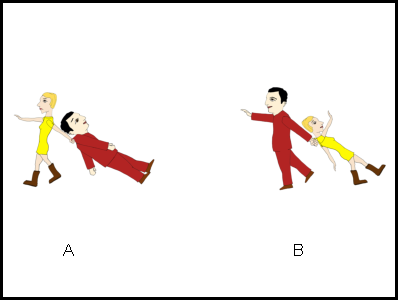
\includegraphics[width=\textwidth]{figures/02-7.pdf}
    \caption{Comprehension test: alternative descriptions of the target utterance}
    \label{fig:02:7}
\end{figure} 

The learners' task was to select the picture which in their opinion best depicted the stimulus sentence. Responses were marked in pen on an answer sheet. The data thus obtained were digitalised manually in spreadsheet format and then further manipulated and analysed with R (\citealt{RCoreTeam2017}).

\paragraph{Comprehension test: target items}

The test comprises 24 target sentences, in addition to three warm-up sentences to make sure that learners had correctly understood its structure. The test was administered collectively in a classroom: target sentences were played aloud through loudspeakers while pictures were projected on screen. Learners took the test after 9 hours (T1) and 13:30 hours (T2) of exposure to the input, consistently with the timing of the EI test described in the preceding chapter: the two tasks probe different aspects of the learner's developing competence in the L2 after identical exposure to the input.

Target sentences had the structure NP - Verb - NP. Only two nouns were used for this test, namely \textit{brat}, ‘brother’, and \textit{siostra}, ‘sister’. The verbs were the same employed in the EIT, namely \textit{ciągnie}, ‘pulls’,  \textit{pcha}, ‘pushes’, \textit{pozdrawia}, ‘greets’, and \textit{woła}, ‘calls’. Each noun appeared in both its NOM and ACC form; further constituent order varied (SVO, OVS, OSV), each occurring in eight target sentences. 

\begin{table}
    \fittable{
    \begin{tabular}{lllllll}
    \lsptoprule
        \textit{siostr-a} & \textit{woła} & \textit{brat-a} & {~~~~~~} &        \textit{brat} & \textit{woła} & \textit{siostr-ę}\\
        sister-\textsc{nom} & calls & brother-\textsc{acc} & &        brother\textsc{.nom} & calls & sister\textsc{{}-acc}\\
        \tablevspace
        \textit{siostr-a} & \textit{brat-a} & \textit{woła} & &        \textit{siostr-ę} & \textit{brat} & \textit{woła}\\
        sister-\textsc{nom} & brother-\textsc{acc} & calls & &        sister-\textsc{acc} & brother\textsc{.nom} & calls\\
        \tablevspace
        \textit{brat-a} & \textit{woła} & \textit{siostr-a} & &        \textit{siostr-ę} & \textit{woła} & \textit{brat}\\
        brother-\textsc{acc} & calls & sister-\textsc{nom} & &        sister-\textsc{acc} & calls & brother.\textsc{nom}\\
    \lspbottomrule
    \end{tabular}
    }
    \caption{Comprehension test, example of target sentences with the verb woła}
    \label{tab:02:14}
\end{table}

\tabref{tab:02:15} presents the relevant forms of the paradigm of the two target nouns employed in the test. \textit{Brat} follows the declension of masculine animate nouns, \textit{siostra} that of feminine nouns in -a.

\begin{table}
    \begin{tabularx}{\textwidth}{XXl}
    \lsptoprule
           & \textit{brat} ‘brother’ & \textit{siostra} ‘sister’\\
    \midrule
        NOM & \textit{brat} & \textit{siostr-a}\\
        ACC & \textit{brat-a} & \textit{siostr-ę}\\
    \lspbottomrule
    \end{tabularx}
    \caption{Comprehension test, paradigm of the target nouns}
    \label{tab:02:15}
\end{table}

As can be seen, the ACC case of masculine nouns like \textit{brat} is characterised by the ending \textit{{}-a}, which also occurs in the NOM case of feminine nouns like \textit{siostra}. This observation will be of some relevance in our subsequent analysis of the data.

\subsection{Semi-spontaneous production}\label{sec:02:4.5}

An essential part of the VILLA experimental protocol consists in the monitoring of learner output during classes. To this end, participants were seated in front of directional microphones which recorded everything they said during the whole course, as illustrated in \figref{fig:02:8}. The entire output of each participant was recorded on a separate track.

\begin{figure}
    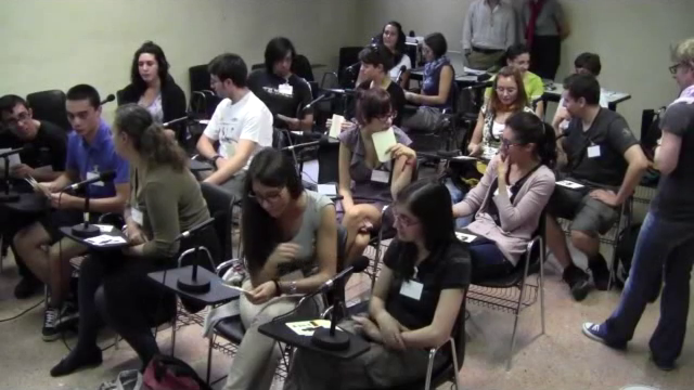
\includegraphics[width=\textwidth]{figures/02-8.pdf}
    \caption{VILLA classroom set-up}
    \label{fig:02:8}
\end{figure}

The VILLA course comprises several dialogic episodes during which participants could interact with each other. They were typically given a simple task to perform in pairs using grammatical structures or vocabulary which had been previously practiced collectively with the teacher. The data presented in this book were collected during one such occasion, which took place during lesson 7.2, after roughly 10:30 hours of exposure to the input. The development of the interlanguage at that stage should be roughly comparable to that probed though the structured tests (the EIT and the Comprehension test) at T1 (lesson 6.2, 9 hours of input exposure). Given the amount of work required to prepare the raw production data for analysis, only a subset of the VILLA data-set could be analysed, i.e. the Italian MB input group.

Participants were divided into 7 groups of 2 and a group of 3. Each group was given a set of cards containing information about several referents that learners were asked to describe to each other. Each card in a learner's set only contained part of the information: the remaining details could be found on the corresponding card in the partner's set, so that, in order to obtain a full description of the referent, information had to be exchanged between the two. While the first participant described the referent based on his or her card, the partner would try to identify the character, asking questions to complete the missing data. In doing so, learners were encouraged to use all structures presented during the course, including the transitive constructions which constitute the object of this work. 

For this study, the fragments relative to the interactive episode were extracted from the track of each participant and merged according to the groups in which learners were divided. Following this operation, each resulting track contained only the speech of the two or three participants who were part of the same group.  The data were then transcribed along the lines described in \sectref{sec:02:4.1} and further divided into one-verb utterances. Synchronised video recordings proved of great help to identify participants, providing the transcriber with an additional clue, in addition to the sound of learners' voices. The resulting corpus comprises 60 utterances produced by 17 learners.
